% Created by tikzDevice version 0.12 on 2019-07-24 04:41:15
% !TEX encoding = UTF-8 Unicode
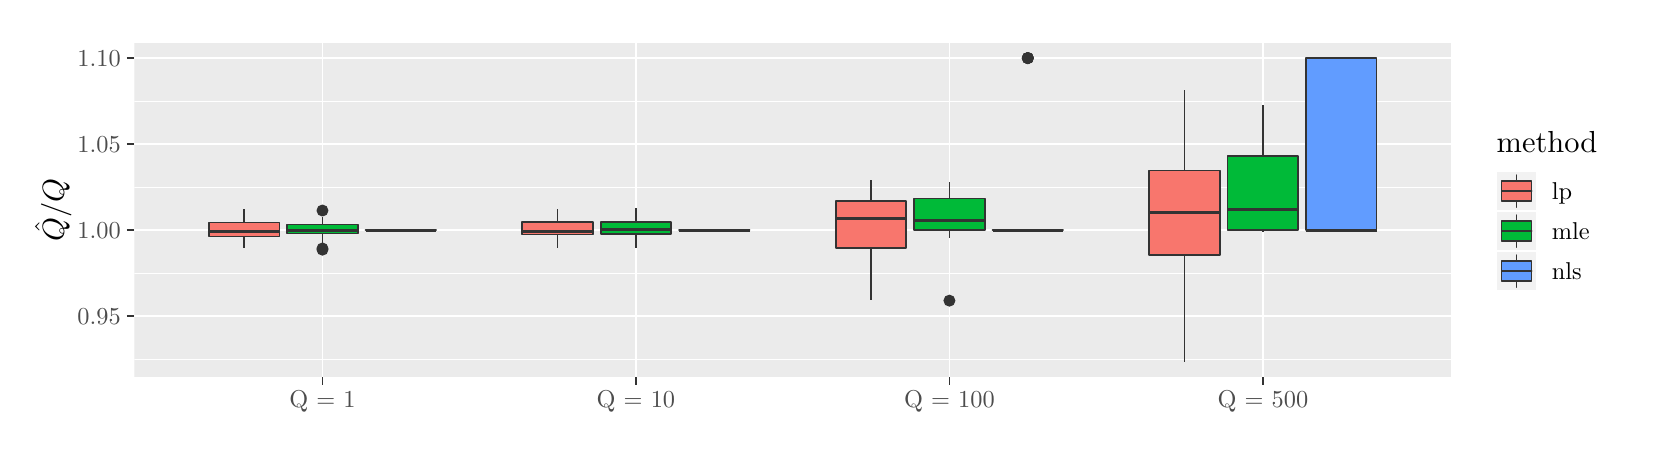
\begin{tikzpicture}[x=1pt,y=1pt]
\definecolor{fillColor}{RGB}{255,255,255}
\path[use as bounding box,fill=fillColor,fill opacity=0.00] (0,0) rectangle (578.16,144.54);
\begin{scope}
\path[clip] (  0.00,  0.00) rectangle (578.16,144.54);
\definecolor{drawColor}{RGB}{255,255,255}
\definecolor{fillColor}{RGB}{255,255,255}

\path[draw=drawColor,line width= 0.6pt,line join=round,line cap=round,fill=fillColor] (  0.00,  0.00) rectangle (578.16,144.54);
\end{scope}
\begin{scope}
\path[clip] ( 38.56, 18.22) rectangle (514.31,139.04);
\definecolor{fillColor}{gray}{0.92}

\path[fill=fillColor] ( 38.56, 18.22) rectangle (514.31,139.04);
\definecolor{drawColor}{RGB}{255,255,255}

\path[draw=drawColor,line width= 0.3pt,line join=round] ( 38.56, 24.80) --
	(514.31, 24.80);

\path[draw=drawColor,line width= 0.3pt,line join=round] ( 38.56, 55.87) --
	(514.31, 55.87);

\path[draw=drawColor,line width= 0.3pt,line join=round] ( 38.56, 86.94) --
	(514.31, 86.94);

\path[draw=drawColor,line width= 0.3pt,line join=round] ( 38.56,118.01) --
	(514.31,118.01);

\path[draw=drawColor,line width= 0.6pt,line join=round] ( 38.56, 40.34) --
	(514.31, 40.34);

\path[draw=drawColor,line width= 0.6pt,line join=round] ( 38.56, 71.41) --
	(514.31, 71.41);

\path[draw=drawColor,line width= 0.6pt,line join=round] ( 38.56,102.48) --
	(514.31,102.48);

\path[draw=drawColor,line width= 0.6pt,line join=round] ( 38.56,133.55) --
	(514.31,133.55);

\path[draw=drawColor,line width= 0.6pt,line join=round] (106.52, 18.22) --
	(106.52,139.04);

\path[draw=drawColor,line width= 0.6pt,line join=round] (219.79, 18.22) --
	(219.79,139.04);

\path[draw=drawColor,line width= 0.6pt,line join=round] (333.07, 18.22) --
	(333.07,139.04);

\path[draw=drawColor,line width= 0.6pt,line join=round] (446.34, 18.22) --
	(446.34,139.04);
\definecolor{drawColor}{gray}{0.20}

\path[draw=drawColor,line width= 0.6pt,line join=round] ( 78.20, 74.15) -- ( 78.20, 78.91);

\path[draw=drawColor,line width= 0.6pt,line join=round] ( 78.20, 69.14) -- ( 78.20, 64.77);
\definecolor{fillColor}{RGB}{248,118,109}

\path[draw=drawColor,line width= 0.6pt,line join=round,line cap=round,fill=fillColor] ( 65.46, 74.15) --
	( 65.46, 69.14) --
	( 90.94, 69.14) --
	( 90.94, 74.15) --
	( 65.46, 74.15) --
	cycle;

\path[draw=drawColor,line width= 1.1pt,line join=round] ( 65.46, 71.04) -- ( 90.94, 71.04);
\definecolor{fillColor}{gray}{0.20}

\path[draw=drawColor,line width= 0.4pt,line join=round,line cap=round,fill=fillColor] (106.52, 78.46) circle (  1.96);

\path[draw=drawColor,line width= 0.4pt,line join=round,line cap=round,fill=fillColor] (106.52, 64.32) circle (  1.96);

\path[draw=drawColor,line width= 0.4pt,line join=round,line cap=round,fill=fillColor] (106.52, 64.75) circle (  1.96);

\path[draw=drawColor,line width= 0.6pt,line join=round] (106.52, 73.45) -- (106.52, 76.18);

\path[draw=drawColor,line width= 0.6pt,line join=round] (106.52, 70.19) -- (106.52, 66.67);
\definecolor{fillColor}{RGB}{0,186,56}

\path[draw=drawColor,line width= 0.6pt,line join=round,line cap=round,fill=fillColor] ( 93.78, 73.45) --
	( 93.78, 70.19) --
	(119.26, 70.19) --
	(119.26, 73.45) --
	( 93.78, 73.45) --
	cycle;

\path[draw=drawColor,line width= 1.1pt,line join=round] ( 93.78, 71.39) -- (119.26, 71.39);

\path[draw=drawColor,line width= 0.6pt,line join=round] (134.84, 71.41) -- (134.84, 71.41);

\path[draw=drawColor,line width= 0.6pt,line join=round] (134.84, 71.41) -- (134.84, 71.41);
\definecolor{fillColor}{RGB}{97,156,255}

\path[draw=drawColor,line width= 0.6pt,line join=round,line cap=round,fill=fillColor] (122.09, 71.41) --
	(122.09, 71.41) --
	(147.58, 71.41) --
	(147.58, 71.41) --
	(122.09, 71.41) --
	cycle;

\path[draw=drawColor,line width= 1.1pt,line join=round] (122.09, 71.41) -- (147.58, 71.41);

\path[draw=drawColor,line width= 0.6pt,line join=round] (191.48, 74.36) -- (191.48, 79.18);

\path[draw=drawColor,line width= 0.6pt,line join=round] (191.48, 69.80) -- (191.48, 64.77);
\definecolor{fillColor}{RGB}{248,118,109}

\path[draw=drawColor,line width= 0.6pt,line join=round,line cap=round,fill=fillColor] (178.73, 74.36) --
	(178.73, 69.80) --
	(204.22, 69.80) --
	(204.22, 74.36) --
	(178.73, 74.36) --
	cycle;

\path[draw=drawColor,line width= 1.1pt,line join=round] (178.73, 71.00) -- (204.22, 71.00);

\path[draw=drawColor,line width= 0.6pt,line join=round] (219.79, 74.34) -- (219.79, 79.48);

\path[draw=drawColor,line width= 0.6pt,line join=round] (219.79, 70.09) -- (219.79, 64.90);
\definecolor{fillColor}{RGB}{0,186,56}

\path[draw=drawColor,line width= 0.6pt,line join=round,line cap=round,fill=fillColor] (207.05, 74.34) --
	(207.05, 70.09) --
	(232.54, 70.09) --
	(232.54, 74.34) --
	(207.05, 74.34) --
	cycle;

\path[draw=drawColor,line width= 1.1pt,line join=round] (207.05, 71.48) -- (232.54, 71.48);

\path[draw=drawColor,line width= 0.6pt,line join=round] (248.11, 71.41) -- (248.11, 71.41);

\path[draw=drawColor,line width= 0.6pt,line join=round] (248.11, 71.41) -- (248.11, 71.41);
\definecolor{fillColor}{RGB}{97,156,255}

\path[draw=drawColor,line width= 0.6pt,line join=round,line cap=round,fill=fillColor] (235.37, 71.41) --
	(235.37, 71.41) --
	(260.86, 71.41) --
	(260.86, 71.41) --
	(235.37, 71.41) --
	cycle;

\path[draw=drawColor,line width= 1.1pt,line join=round] (235.37, 71.41) -- (260.86, 71.41);

\path[draw=drawColor,line width= 0.6pt,line join=round] (304.75, 81.97) -- (304.75, 89.52);

\path[draw=drawColor,line width= 0.6pt,line join=round] (304.75, 64.91) -- (304.75, 45.98);
\definecolor{fillColor}{RGB}{248,118,109}

\path[draw=drawColor,line width= 0.6pt,line join=round,line cap=round,fill=fillColor] (292.01, 81.97) --
	(292.01, 64.91) --
	(317.49, 64.91) --
	(317.49, 81.97) --
	(292.01, 81.97) --
	cycle;

\path[draw=drawColor,line width= 1.1pt,line join=round] (292.01, 75.67) -- (317.49, 75.67);
\definecolor{fillColor}{gray}{0.20}

\path[draw=drawColor,line width= 0.4pt,line join=round,line cap=round,fill=fillColor] (333.07, 45.90) circle (  1.96);

\path[draw=drawColor,line width= 0.6pt,line join=round] (333.07, 82.82) -- (333.07, 88.89);

\path[draw=drawColor,line width= 0.6pt,line join=round] (333.07, 71.41) -- (333.07, 68.49);
\definecolor{fillColor}{RGB}{0,186,56}

\path[draw=drawColor,line width= 0.6pt,line join=round,line cap=round,fill=fillColor] (320.33, 82.82) --
	(320.33, 71.41) --
	(345.81, 71.41) --
	(345.81, 82.82) --
	(320.33, 82.82) --
	cycle;

\path[draw=drawColor,line width= 1.1pt,line join=round] (320.33, 74.81) -- (345.81, 74.81);
\definecolor{fillColor}{gray}{0.20}

\path[draw=drawColor,line width= 0.4pt,line join=round,line cap=round,fill=fillColor] (361.39,133.55) circle (  1.96);

\path[draw=drawColor,line width= 0.4pt,line join=round,line cap=round,fill=fillColor] (361.39,133.55) circle (  1.96);

\path[draw=drawColor,line width= 0.4pt,line join=round,line cap=round,fill=fillColor] (361.39,133.55) circle (  1.96);

\path[draw=drawColor,line width= 0.4pt,line join=round,line cap=round,fill=fillColor] (361.39,133.55) circle (  1.96);

\path[draw=drawColor,line width= 0.6pt,line join=round] (361.39, 71.41) -- (361.39, 71.41);

\path[draw=drawColor,line width= 0.6pt,line join=round] (361.39, 71.41) -- (361.39, 71.41);
\definecolor{fillColor}{RGB}{97,156,255}

\path[draw=drawColor,line width= 0.6pt,line join=round,line cap=round,fill=fillColor] (348.64, 71.41) --
	(348.64, 71.41) --
	(374.13, 71.41) --
	(374.13, 71.41) --
	(348.64, 71.41) --
	cycle;

\path[draw=drawColor,line width= 1.1pt,line join=round] (348.64, 71.41) -- (374.13, 71.41);

\path[draw=drawColor,line width= 0.6pt,line join=round] (418.02, 92.90) -- (418.02,122.03);

\path[draw=drawColor,line width= 0.6pt,line join=round] (418.02, 62.45) -- (418.02, 23.71);
\definecolor{fillColor}{RGB}{248,118,109}

\path[draw=drawColor,line width= 0.6pt,line join=round,line cap=round,fill=fillColor] (405.28, 92.90) --
	(405.28, 62.45) --
	(430.77, 62.45) --
	(430.77, 92.90) --
	(405.28, 92.90) --
	cycle;

\path[draw=drawColor,line width= 1.1pt,line join=round] (405.28, 77.75) -- (430.77, 77.75);

\path[draw=drawColor,line width= 0.6pt,line join=round] (446.34, 98.09) -- (446.34,116.44);

\path[draw=drawColor,line width= 0.6pt,line join=round] (446.34, 71.52) -- (446.34, 70.79);
\definecolor{fillColor}{RGB}{0,186,56}

\path[draw=drawColor,line width= 0.6pt,line join=round,line cap=round,fill=fillColor] (433.60, 98.09) --
	(433.60, 71.52) --
	(459.09, 71.52) --
	(459.09, 98.09) --
	(433.60, 98.09) --
	cycle;

\path[draw=drawColor,line width= 1.1pt,line join=round] (433.60, 78.93) -- (459.09, 78.93);

\path[draw=drawColor,line width= 0.6pt,line join=round] (474.66,133.55) -- (474.66,133.55);

\path[draw=drawColor,line width= 0.6pt,line join=round] (474.66, 71.41) -- (474.66, 71.41);
\definecolor{fillColor}{RGB}{97,156,255}

\path[draw=drawColor,line width= 0.6pt,line join=round,line cap=round,fill=fillColor] (461.92,133.55) --
	(461.92, 71.41) --
	(487.40, 71.41) --
	(487.40,133.55) --
	(461.92,133.55) --
	cycle;

\path[draw=drawColor,line width= 1.1pt,line join=round] (461.92, 71.41) -- (487.40, 71.41);
\end{scope}
\begin{scope}
\path[clip] (  0.00,  0.00) rectangle (578.16,144.54);
\definecolor{drawColor}{gray}{0.30}

\node[text=drawColor,anchor=base east,inner sep=0pt, outer sep=0pt, scale=  0.88] at ( 33.61, 37.31) {0.95};

\node[text=drawColor,anchor=base east,inner sep=0pt, outer sep=0pt, scale=  0.88] at ( 33.61, 68.38) {1.00};

\node[text=drawColor,anchor=base east,inner sep=0pt, outer sep=0pt, scale=  0.88] at ( 33.61, 99.45) {1.05};

\node[text=drawColor,anchor=base east,inner sep=0pt, outer sep=0pt, scale=  0.88] at ( 33.61,130.52) {1.10};
\end{scope}
\begin{scope}
\path[clip] (  0.00,  0.00) rectangle (578.16,144.54);
\definecolor{drawColor}{gray}{0.20}

\path[draw=drawColor,line width= 0.6pt,line join=round] ( 35.81, 40.34) --
	( 38.56, 40.34);

\path[draw=drawColor,line width= 0.6pt,line join=round] ( 35.81, 71.41) --
	( 38.56, 71.41);

\path[draw=drawColor,line width= 0.6pt,line join=round] ( 35.81,102.48) --
	( 38.56,102.48);

\path[draw=drawColor,line width= 0.6pt,line join=round] ( 35.81,133.55) --
	( 38.56,133.55);
\end{scope}
\begin{scope}
\path[clip] (  0.00,  0.00) rectangle (578.16,144.54);
\definecolor{drawColor}{gray}{0.20}

\path[draw=drawColor,line width= 0.6pt,line join=round] (106.52, 15.47) --
	(106.52, 18.22);

\path[draw=drawColor,line width= 0.6pt,line join=round] (219.79, 15.47) --
	(219.79, 18.22);

\path[draw=drawColor,line width= 0.6pt,line join=round] (333.07, 15.47) --
	(333.07, 18.22);

\path[draw=drawColor,line width= 0.6pt,line join=round] (446.34, 15.47) --
	(446.34, 18.22);
\end{scope}
\begin{scope}
\path[clip] (  0.00,  0.00) rectangle (578.16,144.54);
\definecolor{drawColor}{gray}{0.30}

\node[text=drawColor,anchor=base,inner sep=0pt, outer sep=0pt, scale=  0.88] at (106.52,  7.21) {Q = 1};

\node[text=drawColor,anchor=base,inner sep=0pt, outer sep=0pt, scale=  0.88] at (219.79,  7.21) {Q = 10};

\node[text=drawColor,anchor=base,inner sep=0pt, outer sep=0pt, scale=  0.88] at (333.07,  7.21) {Q = 100};

\node[text=drawColor,anchor=base,inner sep=0pt, outer sep=0pt, scale=  0.88] at (446.34,  7.21) {Q = 500};
\end{scope}
\begin{scope}
\path[clip] (  0.00,  0.00) rectangle (578.16,144.54);
\definecolor{drawColor}{RGB}{0,0,0}

\node[text=drawColor,rotate= 90.00,anchor=base,inner sep=0pt, outer sep=0pt, scale=  1.10] at ( 13.08, 78.63) {$\hat{Q}/Q$};
\end{scope}
\begin{scope}
\path[clip] (  0.00,  0.00) rectangle (578.16,144.54);
\definecolor{fillColor}{RGB}{255,255,255}

\path[fill=fillColor] (525.31, 43.84) rectangle (572.66,113.42);
\end{scope}
\begin{scope}
\path[clip] (  0.00,  0.00) rectangle (578.16,144.54);
\definecolor{drawColor}{RGB}{0,0,0}

\node[text=drawColor,anchor=base west,inner sep=0pt, outer sep=0pt, scale=  1.10] at (530.81, 99.27) {method};
\end{scope}
\begin{scope}
\path[clip] (  0.00,  0.00) rectangle (578.16,144.54);
\definecolor{drawColor}{RGB}{255,255,255}
\definecolor{fillColor}{gray}{0.95}

\path[draw=drawColor,line width= 0.6pt,line join=round,line cap=round,fill=fillColor] (530.81, 78.25) rectangle (545.26, 92.70);
\end{scope}
\begin{scope}
\path[clip] (  0.00,  0.00) rectangle (578.16,144.54);
\definecolor{drawColor}{gray}{0.20}

\path[draw=drawColor,line width= 0.6pt,line join=round,line cap=round] (538.03, 79.70) --
	(538.03, 81.86);

\path[draw=drawColor,line width= 0.6pt,line join=round,line cap=round] (538.03, 89.09) --
	(538.03, 91.26);
\definecolor{fillColor}{RGB}{248,118,109}

\path[draw=drawColor,line width= 0.6pt,line join=round,line cap=round,fill=fillColor] (532.61, 81.86) rectangle (543.45, 89.09);

\path[draw=drawColor,line width= 0.6pt,line join=round,line cap=round] (532.61, 85.48) --
	(543.45, 85.48);
\end{scope}
\begin{scope}
\path[clip] (  0.00,  0.00) rectangle (578.16,144.54);
\definecolor{drawColor}{RGB}{255,255,255}
\definecolor{fillColor}{gray}{0.95}

\path[draw=drawColor,line width= 0.6pt,line join=round,line cap=round,fill=fillColor] (530.81, 63.80) rectangle (545.26, 78.25);
\end{scope}
\begin{scope}
\path[clip] (  0.00,  0.00) rectangle (578.16,144.54);
\definecolor{drawColor}{gray}{0.20}

\path[draw=drawColor,line width= 0.6pt,line join=round,line cap=round] (538.03, 65.24) --
	(538.03, 67.41);

\path[draw=drawColor,line width= 0.6pt,line join=round,line cap=round] (538.03, 74.64) --
	(538.03, 76.81);
\definecolor{fillColor}{RGB}{0,186,56}

\path[draw=drawColor,line width= 0.6pt,line join=round,line cap=round,fill=fillColor] (532.61, 67.41) rectangle (543.45, 74.64);

\path[draw=drawColor,line width= 0.6pt,line join=round,line cap=round] (532.61, 71.02) --
	(543.45, 71.02);
\end{scope}
\begin{scope}
\path[clip] (  0.00,  0.00) rectangle (578.16,144.54);
\definecolor{drawColor}{RGB}{255,255,255}
\definecolor{fillColor}{gray}{0.95}

\path[draw=drawColor,line width= 0.6pt,line join=round,line cap=round,fill=fillColor] (530.81, 49.34) rectangle (545.26, 63.80);
\end{scope}
\begin{scope}
\path[clip] (  0.00,  0.00) rectangle (578.16,144.54);
\definecolor{drawColor}{gray}{0.20}

\path[draw=drawColor,line width= 0.6pt,line join=round,line cap=round] (538.03, 50.79) --
	(538.03, 52.96);

\path[draw=drawColor,line width= 0.6pt,line join=round,line cap=round] (538.03, 60.18) --
	(538.03, 62.35);
\definecolor{fillColor}{RGB}{97,156,255}

\path[draw=drawColor,line width= 0.6pt,line join=round,line cap=round,fill=fillColor] (532.61, 52.96) rectangle (543.45, 60.18);

\path[draw=drawColor,line width= 0.6pt,line join=round,line cap=round] (532.61, 56.57) --
	(543.45, 56.57);
\end{scope}
\begin{scope}
\path[clip] (  0.00,  0.00) rectangle (578.16,144.54);
\definecolor{drawColor}{RGB}{0,0,0}

\node[text=drawColor,anchor=base west,inner sep=0pt, outer sep=0pt, scale=  0.88] at (550.76, 82.45) {lp};
\end{scope}
\begin{scope}
\path[clip] (  0.00,  0.00) rectangle (578.16,144.54);
\definecolor{drawColor}{RGB}{0,0,0}

\node[text=drawColor,anchor=base west,inner sep=0pt, outer sep=0pt, scale=  0.88] at (550.76, 67.99) {mle};
\end{scope}
\begin{scope}
\path[clip] (  0.00,  0.00) rectangle (578.16,144.54);
\definecolor{drawColor}{RGB}{0,0,0}

\node[text=drawColor,anchor=base west,inner sep=0pt, outer sep=0pt, scale=  0.88] at (550.76, 53.54) {nls};
\end{scope}
\end{tikzpicture}
